% Options for packages loaded elsewhere
\PassOptionsToPackage{unicode}{hyperref}
\PassOptionsToPackage{hyphens}{url}
\PassOptionsToPackage{dvipsnames,svgnames*,x11names*}{xcolor}
%
\documentclass[
  12pt,
]{krantz}
\usepackage{lmodern}
\usepackage{amssymb,amsmath}
\usepackage{ifxetex,ifluatex}
\ifnum 0\ifxetex 1\fi\ifluatex 1\fi=0 % if pdftex
  \usepackage[T1]{fontenc}
  \usepackage[utf8]{inputenc}
  \usepackage{textcomp} % provide euro and other symbols
\else % if luatex or xetex
  \usepackage{unicode-math}
  \defaultfontfeatures{Scale=MatchLowercase}
  \defaultfontfeatures[\rmfamily]{Ligatures=TeX,Scale=1}
  \setmonofont[Scale=0.7]{Source Code Pro}
\fi
% Use upquote if available, for straight quotes in verbatim environments
\IfFileExists{upquote.sty}{\usepackage{upquote}}{}
\IfFileExists{microtype.sty}{% use microtype if available
  \usepackage[]{microtype}
  \UseMicrotypeSet[protrusion]{basicmath} % disable protrusion for tt fonts
}{}
\makeatletter
\@ifundefined{KOMAClassName}{% if non-KOMA class
  \IfFileExists{parskip.sty}{%
    \usepackage{parskip}
  }{% else
    \setlength{\parindent}{0pt}
    \setlength{\parskip}{6pt plus 2pt minus 1pt}}
}{% if KOMA class
  \KOMAoptions{parskip=half}}
\makeatother
\usepackage{xcolor}
\IfFileExists{xurl.sty}{\usepackage{xurl}}{} % add URL line breaks if available
\IfFileExists{bookmark.sty}{\usepackage{bookmark}}{\usepackage{hyperref}}
\hypersetup{
  pdftitle={nmw: R패키지와 Edison 사이언스 앱을 이용한 비선형 혼합효과 모델링과 시뮬레이션},
  pdfauthor={한성필, 조용순, 김형섭, 배균섭},
  colorlinks=true,
  linkcolor=Maroon,
  filecolor=Maroon,
  citecolor=Blue,
  urlcolor=Blue,
  pdfcreator={LaTeX via pandoc}}
\urlstyle{same} % disable monospaced font for URLs
\usepackage{color}
\usepackage{fancyvrb}
\newcommand{\VerbBar}{|}
\newcommand{\VERB}{\Verb[commandchars=\\\{\}]}
\DefineVerbatimEnvironment{Highlighting}{Verbatim}{commandchars=\\\{\}}
% Add ',fontsize=\small' for more characters per line
\usepackage{framed}
\definecolor{shadecolor}{RGB}{248,248,248}
\newenvironment{Shaded}{\begin{snugshade}}{\end{snugshade}}
\newcommand{\AlertTok}[1]{\textcolor[rgb]{0.94,0.16,0.16}{#1}}
\newcommand{\AnnotationTok}[1]{\textcolor[rgb]{0.56,0.35,0.01}{\textbf{\textit{#1}}}}
\newcommand{\AttributeTok}[1]{\textcolor[rgb]{0.77,0.63,0.00}{#1}}
\newcommand{\BaseNTok}[1]{\textcolor[rgb]{0.00,0.00,0.81}{#1}}
\newcommand{\BuiltInTok}[1]{#1}
\newcommand{\CharTok}[1]{\textcolor[rgb]{0.31,0.60,0.02}{#1}}
\newcommand{\CommentTok}[1]{\textcolor[rgb]{0.56,0.35,0.01}{\textit{#1}}}
\newcommand{\CommentVarTok}[1]{\textcolor[rgb]{0.56,0.35,0.01}{\textbf{\textit{#1}}}}
\newcommand{\ConstantTok}[1]{\textcolor[rgb]{0.00,0.00,0.00}{#1}}
\newcommand{\ControlFlowTok}[1]{\textcolor[rgb]{0.13,0.29,0.53}{\textbf{#1}}}
\newcommand{\DataTypeTok}[1]{\textcolor[rgb]{0.13,0.29,0.53}{#1}}
\newcommand{\DecValTok}[1]{\textcolor[rgb]{0.00,0.00,0.81}{#1}}
\newcommand{\DocumentationTok}[1]{\textcolor[rgb]{0.56,0.35,0.01}{\textbf{\textit{#1}}}}
\newcommand{\ErrorTok}[1]{\textcolor[rgb]{0.64,0.00,0.00}{\textbf{#1}}}
\newcommand{\ExtensionTok}[1]{#1}
\newcommand{\FloatTok}[1]{\textcolor[rgb]{0.00,0.00,0.81}{#1}}
\newcommand{\FunctionTok}[1]{\textcolor[rgb]{0.00,0.00,0.00}{#1}}
\newcommand{\ImportTok}[1]{#1}
\newcommand{\InformationTok}[1]{\textcolor[rgb]{0.56,0.35,0.01}{\textbf{\textit{#1}}}}
\newcommand{\KeywordTok}[1]{\textcolor[rgb]{0.13,0.29,0.53}{\textbf{#1}}}
\newcommand{\NormalTok}[1]{#1}
\newcommand{\OperatorTok}[1]{\textcolor[rgb]{0.81,0.36,0.00}{\textbf{#1}}}
\newcommand{\OtherTok}[1]{\textcolor[rgb]{0.56,0.35,0.01}{#1}}
\newcommand{\PreprocessorTok}[1]{\textcolor[rgb]{0.56,0.35,0.01}{\textit{#1}}}
\newcommand{\RegionMarkerTok}[1]{#1}
\newcommand{\SpecialCharTok}[1]{\textcolor[rgb]{0.00,0.00,0.00}{#1}}
\newcommand{\SpecialStringTok}[1]{\textcolor[rgb]{0.31,0.60,0.02}{#1}}
\newcommand{\StringTok}[1]{\textcolor[rgb]{0.31,0.60,0.02}{#1}}
\newcommand{\VariableTok}[1]{\textcolor[rgb]{0.00,0.00,0.00}{#1}}
\newcommand{\VerbatimStringTok}[1]{\textcolor[rgb]{0.31,0.60,0.02}{#1}}
\newcommand{\WarningTok}[1]{\textcolor[rgb]{0.56,0.35,0.01}{\textbf{\textit{#1}}}}
\usepackage{longtable,booktabs}
% Correct order of tables after \paragraph or \subparagraph
\usepackage{etoolbox}
\makeatletter
\patchcmd\longtable{\par}{\if@noskipsec\mbox{}\fi\par}{}{}
\makeatother
% Allow footnotes in longtable head/foot
\IfFileExists{footnotehyper.sty}{\usepackage{footnotehyper}}{\usepackage{footnote}}
\makesavenoteenv{longtable}
\usepackage{graphicx}
\makeatletter
\def\maxwidth{\ifdim\Gin@nat@width>\linewidth\linewidth\else\Gin@nat@width\fi}
\def\maxheight{\ifdim\Gin@nat@height>\textheight\textheight\else\Gin@nat@height\fi}
\makeatother
% Scale images if necessary, so that they will not overflow the page
% margins by default, and it is still possible to overwrite the defaults
% using explicit options in \includegraphics[width, height, ...]{}
\setkeys{Gin}{width=\maxwidth,height=\maxheight,keepaspectratio}
% Set default figure placement to htbp
\makeatletter
\def\fps@figure{htbp}
\makeatother
\setlength{\emergencystretch}{3em} % prevent overfull lines
\providecommand{\tightlist}{%
  \setlength{\itemsep}{0pt}\setlength{\parskip}{0pt}}
\setcounter{secnumdepth}{5}
\usepackage{kotex}

% 이 위로 성필

\usepackage{booktabs}
\usepackage{longtable}
\usepackage[bf,singlelinecheck=off]{caption}

\setmainfont[UprightFeatures={SmallCapsFont=AlegreyaSC-Regular}]{Alegreya}

\usepackage{framed,color}
\definecolor{shadecolor}{RGB}{248,248,248}

\renewcommand{\textfraction}{0.05}
\renewcommand{\topfraction}{0.8}
\renewcommand{\bottomfraction}{0.8}
\renewcommand{\floatpagefraction}{0.75}

\renewenvironment{quote}{\begin{VF}}{\end{VF}}
\let\oldhref\href
\renewcommand{\href}[2]{#2\footnote{\url{#1}}}

\ifxetex
  \usepackage{letltxmacro}
  \setlength{\XeTeXLinkMargin}{1pt}
  \LetLtxMacro\SavedIncludeGraphics\includegraphics
  \def\includegraphics#1#{% #1 catches optional stuff (star/opt. arg.)
    \IncludeGraphicsAux{#1}%
  }%
  \newcommand*{\IncludeGraphicsAux}[2]{%
    \XeTeXLinkBox{%
      \SavedIncludeGraphics#1{#2}%
    }%
  }%
\fi

\makeatletter
\newenvironment{kframe}{%
\medskip{}
\setlength{\fboxsep}{.8em}
 \def\at@end@of@kframe{}%
 \ifinner\ifhmode%
  \def\at@end@of@kframe{\end{minipage}}%
  \begin{minipage}{\columnwidth}%
 \fi\fi%
 \def\FrameCommand##1{\hskip\@totalleftmargin \hskip-\fboxsep
 \colorbox{shadecolor}{##1}\hskip-\fboxsep
     % There is no \\@totalrightmargin, so:
     \hskip-\linewidth \hskip-\@totalleftmargin \hskip\columnwidth}%
 \MakeFramed {\advance\hsize-\width
   \@totalleftmargin\z@ \linewidth\hsize
   \@setminipage}}%
 {\par\unskip\endMakeFramed%
 \at@end@of@kframe}
\makeatother

\renewenvironment{Shaded}{\begin{kframe}}{\end{kframe}}

\newenvironment{rmdblock}[1]
  {
  \begin{itemize}
  \renewcommand{\labelitemi}{
    \raisebox{-.7\height}[0pt][0pt]{
      {\setkeys{Gin}{width=3em,keepaspectratio}\includegraphics{images/#1}}
    }
  }
  \setlength{\fboxsep}{1em}
  \begin{kframe}
  \item
  }
  {
  \end{kframe}
  \end{itemize}
  }
\newenvironment{rmdnote}
  {\begin{rmdblock}{note}}
  {\end{rmdblock}}
\newenvironment{rmdcaution}
  {\begin{rmdblock}{caution}}
  {\end{rmdblock}}
\newenvironment{rmdimportant}
  {\begin{rmdblock}{important}}
  {\end{rmdblock}}
\newenvironment{rmdtip}
  {\begin{rmdblock}{tip}}
  {\end{rmdblock}}
\newenvironment{rmdwarning}
  {\begin{rmdblock}{warning}}
  {\end{rmdblock}}

\usepackage{makeidx}
\makeindex

\urlstyle{tt}

\usepackage{amsthm}
\makeatletter
\def\thm@space@setup{%
  \thm@preskip=8pt plus 2pt minus 4pt
  \thm@postskip=\thm@preskip
}
\makeatother

\frontmatter
\usepackage{booktabs}
\usepackage{longtable}
\usepackage{array}
\usepackage{multirow}
\usepackage{wrapfig}
\usepackage{float}
\usepackage{colortbl}
\usepackage{pdflscape}
\usepackage{tabu}
\usepackage{threeparttable}
\usepackage{threeparttablex}
\usepackage[normalem]{ulem}
\usepackage{makecell}
\usepackage{xcolor}
\usepackage[]{natbib}
\bibliographystyle{apalike}

\title{nmw: R패키지와 Edison 사이언스 앱을 이용한 비선형 혼합효과 모델링과 시뮬레이션}
\author{한성필, 조용순, 김형섭, 배균섭}
\date{2020-05-20}

\begin{document}
\maketitle

%\cleardoublepage\newpage\thispagestyle{empty}\null
%\cleardoublepage\newpage\thispagestyle{empty}\null
%\cleardoublepage\newpage
\thispagestyle{empty}
\begin{center}
%\includegraphics{images/dedication.pdf}
\end{center}

\setlength{\abovedisplayskip}{-5pt}
\setlength{\abovedisplayshortskip}{-5pt}

{
\hypersetup{linkcolor=}
\setcounter{tocdepth}{2}
\tableofcontents
}
\listoftables
\listoffigures
\hypertarget{uxcc45uxba38uxb9acuxc5d0}{%
\chapter*{책머리에}\label{uxcc45uxba38uxb9acuxc5d0}}


본 연구의 목적은 비선형 혼합효과 모델링 과정을 이해하고자 개발된 R패키지의 사용법을 소개하고 이를 활용한 Edison 사이언스앱의 활용법을 제시하는 것입니다. \texttt{nmw} R Package의 기본적인 원리를 설명하고, R 패키지의 함수 사용법을 보이며, 에디슨 앱에서 구현된 활용 예시를 논하고자 합니다. 이를 바탕으로 비선형 혼합효과 모델링의 원리를 익힐 수 있고, 더 나아가 약물의 용법/용량, 모델 파라미터의 변화에 따른 혈중농도 등의 약동학 변화에 대한 다양한 시뮬레이션으로 응용될 수 있습니다.

한성필\textsuperscript{1}, 조용순\textsuperscript{2}, 김형섭\textsuperscript{2}, 배균섭\textsuperscript{2}\\
\textsuperscript{1} 가톨릭대학교 약리학교실
\textsuperscript{2} 서울아산병원 임상약리학과, 울산대학교병원, 서울특별시 송파구 올림픽로43길 88\\
E-mail: 한성필 \href{mailto:shan@catholic.ac.kr}{\nolinkurl{shan@catholic.ac.kr}}, 배균섭 \href{mailto:ksbae@acp.kr}{\nolinkurl{ksbae@acp.kr}}

\mainmatter

\hypertarget{intro}{%
\chapter{서론}\label{intro}}

비선형 혼합효과 모델링(Nonlinear mixed effect modeling)을 위해 가장 흔히 쓰이는 도구는 NONMEM®이라고 하는 소프트웨어입니다. 현재 모델기반 약물개발 (Model-based drug development)를 위한 계량약리학 분야에서 가장 표준적인 도구로 생각되고 있으나 그 동작하는 원리를 이해하기는 쉽지 않습니다. 공개소프트웨어인 R을 통해서 NONMEM의 계산과 알고리듬을 구현하는 시도가 있었고, 성공적으로 결과값을 재현할 수 있음을 보였습니다. \citep{kim2015r, bae2016r} 이 연구를 통해서 NONMEM의 동작원리를 단계별로 실행하며 학습할 수 있게 되었으며, 더 나아가 저자들은 공개 소프트웨어인 nmw R 패키지를 개발 \citep{R-nmw}, 배포하여 이러한 원리를 누구나 비용없이 접근할 수 있게 하였습니다.

\hypertarget{method}{%
\chapter{이론 및 계산방법}\label{method}}

\hypertarget{maximum-likelihood-estimation}{%
\section{Maximum Likelihood Estimation}\label{maximum-likelihood-estimation}}

우도함수를 최대화하면서 모수를 추정하는 방법입니다.
관측된 표본에 기초하여 관측 불가능한 파라미터(모수)를 추정하는 방법론 중 하나로, 표본들로부터 알려지지 않은 모집단 확률분포의 형태를 추정해가는 방법론입니다. (An estimation method that finds a combination of parameters which maximizes the likelihood of an observation dataset)

MLE는 주어진 Dataset(관측결과, D)의 발생 가능성(Likelihood, 우도)이 가장 높은 모수를 추정하고, 이를 바탕으로 최적의 f를 도출합니다. 이를 수식으로 표현하면 다음과 같습니다.

정규분포의 경우 n\textsubscript{i}개의 관찰값을 갖는 대상 i에 대해서 -2 log likelihood (-2LL)은 다음과 같이 표현할 수 있습니다.

\[
-2LL_i = n_i \cdot log(2\pi) + \sum\limits_{j=1}^{n_i} log(\sigma_{ij}^2) + \sum\limits_{j=1}^{n_i} \frac{(y_{ij} - \mu_{ij})^2}{\sigma_{ij}^2}
\]

위 함수를 최소화 (우도를 최대화) 하는 모수의 조합은 무엇일까요? 그 결과가 maximum likelihood estimator/estimate (MLE)이고 그 목적함수는 다음과 같습니다.

\[
O_i = \sum\limits_{j=1}^{n_i} log(\sigma_{ij}^2) + \sum\limits_{j=1}^{n_i} \frac{(y_{ij} - \mu_{ij})^2}{\sigma_{ij}^2}
\]

MLE의 장점은 매우 직관적이라는 점입니다. 그리고 별다른 가정을 하지 않고 주어진 관측결과를 바탕으로 쉽계 계산할 수 있습니다. (물론, 관측결과가 이항분포를 따를 것이라는 가정이 들어갔지만, 다른 추정법에 비해서는 가정이 약한 편입니다.)

MLE는 빈도론을 기반으로 합니다. 관측결과에 의존해서 판단하기 때문에 관측결과의 크기(관측횟수)와 질(관측결과의 정확성)에 따라서 모수 추정의 성패가 크게 좌우됩니다.

\hypertarget{first-order-conditional-estimation-foce-method}{%
\section{First-order conditional estimation (FOCE) method}\label{first-order-conditional-estimation-foce-method}}

FOCE는 FO 가정법보다 더 복잡합니다. EBE를 각 iteration 마다 추정하기 때문입니다.

\begin{quote}
The FOCE is more complex than the first-order (FO) approximation method because it estimates the empirical Bayes estimate (EBE) for each iteration. By contrast, it is a further approximation of the Laplacian (LAPL) method, which uses second-order expansion terms. FOCE without INTERACTION can only be used for an additive error model, while FOCE with INTERACTION (FOCEI) can be used for any error model. The formula for FOCE without INTERACTION can be derived directly from the extension of the FO method, while the FOCE with INTERACTION method is a slight simplification of the LAPL method. Detailed formulas and R scripts are presented here for the reproduction of objective function values by NONMEM.
\end{quote}

\hypertarget{uxc124uxce58}{%
\section{설치}\label{uxc124uxce58}}

먼저 R 패키지의 설치 및 로딩 과정은 다음의 명령어를 R 콘솔에 입력함으로서 가능합니다.
NONMEM Workshop 2017에서 사용된 nmw 패키지입니다. \citep{kim2015r, bae2016r, R-nmw}

\begin{Shaded}
\begin{Highlighting}[]
\KeywordTok{install.packages}\NormalTok{(}\StringTok{\textquotesingle{}nmw\textquotesingle{}}\NormalTok{)}
\KeywordTok{library}\NormalTok{(nmw)}
\end{Highlighting}
\end{Shaded}

NONMEM을 통해 얻은 \texttt{THEO-FO.OUT}와 비교할 때 값이 같습니다.

Scaling factor는 소스 코드를 보고 알아낸 것입니다.

\hypertarget{uxc790uxb8cc}{%
\section{자료}\label{uxc790uxb8cc}}

\begin{Shaded}
\begin{Highlighting}[]
\NormalTok{DataAll \textless{}{-}}\StringTok{ }\NormalTok{Theoph}
\KeywordTok{colnames}\NormalTok{(DataAll) \textless{}{-}}\StringTok{ }\KeywordTok{c}\NormalTok{(}\StringTok{"ID"}\NormalTok{, }\StringTok{"BWT"}\NormalTok{, }\StringTok{"DOSE"}\NormalTok{, }\StringTok{"TIME"}\NormalTok{, }\StringTok{"DV"}\NormalTok{)}
\NormalTok{DataAll[,}\StringTok{"ID"}\NormalTok{] \textless{}{-}}\StringTok{ }\KeywordTok{as.numeric}\NormalTok{(}\KeywordTok{as.character}\NormalTok{(DataAll[,}\StringTok{"ID"}\NormalTok{]))}
\end{Highlighting}
\end{Shaded}

이후 \texttt{?nmw} 명령어를 통해 내장되어 있는 예제를 볼 수 있고 이를 실행해 볼 수 있습니다. 사용되는 자료는 R에 내장되어 있는 Theoph이며 이 자료는 12명의 환자에서 테오필린 320 mg을 경구 투여한 후 24시간 동안 혈장에서 측정한 농도를 포함하고 있습니다. 그림을 그려보면 다음과 같습니다. (Figure \ref{fig:xyplot})

\begin{Shaded}
\begin{Highlighting}[]
\NormalTok{lattice}\OperatorTok{::}\KeywordTok{xyplot}\NormalTok{(DV }\OperatorTok{\textasciitilde{}}\StringTok{ }\NormalTok{TIME }\OperatorTok{|}\StringTok{ }\KeywordTok{as.factor}\NormalTok{(ID), }\DataTypeTok{data=}\NormalTok{DataAll, }\DataTypeTok{type=}\StringTok{"b"}\NormalTok{)}
\end{Highlighting}
\end{Shaded}

\begin{figure}
\centering
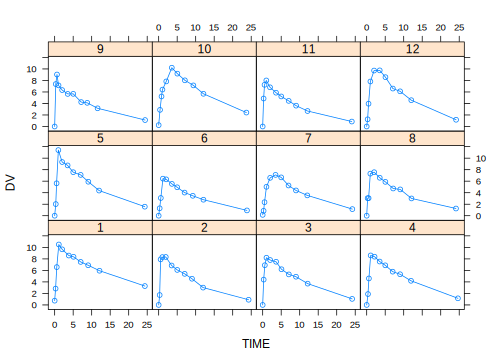
\includegraphics{nmw_files/figure-latex/xyplot-1.pdf}
\caption{\label{fig:xyplot}R에 내장된 Theoph 자료. 이 자료를 사용하여 분석을 시행하였습니다.}
\end{figure}



\begin{Shaded}
\begin{Highlighting}[]
\NormalTok{nTheta =}\StringTok{ }\DecValTok{3}
\NormalTok{nEta =}\StringTok{ }\DecValTok{3}
\NormalTok{nEps =}\StringTok{ }\DecValTok{2}

\NormalTok{THETAinit =}\StringTok{ }\KeywordTok{c}\NormalTok{(}\DecValTok{2}\NormalTok{, }\DecValTok{50}\NormalTok{, }\FloatTok{0.1}\NormalTok{) }
\NormalTok{OMinit =}\StringTok{ }\KeywordTok{matrix}\NormalTok{(}\KeywordTok{c}\NormalTok{(}\FloatTok{0.2}\NormalTok{, }\FloatTok{0.1}\NormalTok{, }\FloatTok{0.1}\NormalTok{, }\FloatTok{0.1}\NormalTok{, }\FloatTok{0.2}\NormalTok{, }\FloatTok{0.1}\NormalTok{, }\FloatTok{0.1}\NormalTok{, }\FloatTok{0.1}\NormalTok{, }\FloatTok{0.2}\NormalTok{), }
                \DataTypeTok{nrow=}\NormalTok{nEta, }\DataTypeTok{ncol=}\NormalTok{nEta)}
\NormalTok{SGinit =}\StringTok{ }\KeywordTok{diag}\NormalTok{(}\KeywordTok{c}\NormalTok{(}\FloatTok{0.1}\NormalTok{, }\FloatTok{0.1}\NormalTok{))}

\NormalTok{LB =}\StringTok{ }\KeywordTok{rep}\NormalTok{(}\DecValTok{0}\NormalTok{, nTheta) }\CommentTok{\# Lower bound}
\NormalTok{UB =}\StringTok{ }\KeywordTok{rep}\NormalTok{(}\DecValTok{1000000}\NormalTok{, nTheta) }\CommentTok{\# Upper bound}
\end{Highlighting}
\end{Shaded}

위 코드는 같이 θ (nTheta), η (nEta), ϵ (nEps)개수를 먼저 지정하고 초기값 (THETAinit, OMinit, SGinit)을 설정하는 과정이며 LB, UB는 θ값 추정의 상한값과 하한값을 정해주는 것으로 적합 (fit)을 성공적으로 수행하기 위해 적절한 범위를 지정해야 합니다. 초기값, 하한값, 상한값은 InitStep() 함수의 인자로 입력되어 initialization step에 사용됩니다. (Figure 2) 이때 PRED 함수 (Figure 3)도 InitStep()의 입력 인자로 사용되는데, 이는 약동학 모델을 미분방정식 형태로 구현한 함수입니다. \{\citet{kang2012standard}\}

InitStep()의 추정방식으로 세가지가 지원되며 ZERO (First Order Approximation Method), COND (First Order Conditional Estimation with Interaction Method), LAPL(Laplacian Approximation with Interacton Method) 에 따라 PRED 함수의 추정 방법이 달라지게 됩니다. {[}1, 2{]} 이후 EstStep(), CovStep(), PostHocEta(), TabStep() 함수를 실행하며 계산을 수행해 나가고 각 함수에 대해 Table 1에서 설명하였습니다.

\begin{Shaded}
\begin{Highlighting}[]
\CommentTok{\#\#\#\#\#\#\#\#\# First Order Approximation Method}
\KeywordTok{InitStep}\NormalTok{(DataAll, }\DataTypeTok{THETAinit=}\NormalTok{THETAinit, }\DataTypeTok{OMinit=}\NormalTok{OMinit, }\DataTypeTok{SGinit=}\NormalTok{SGinit, }
         \DataTypeTok{LB=}\NormalTok{LB, }\DataTypeTok{UB=}\NormalTok{UB, }\DataTypeTok{Pred=}\NormalTok{PRED, }\DataTypeTok{METHOD=}\StringTok{"ZERO"}\NormalTok{)}
\NormalTok{(}\DataTypeTok{EstRes =} \KeywordTok{EstStep}\NormalTok{())           }\CommentTok{\# 4 sec}
\NormalTok{(}\DataTypeTok{CovRes =} \KeywordTok{CovStep}\NormalTok{())           }\CommentTok{\# 2 sec}
\KeywordTok{PostHocEta}\NormalTok{() }\CommentTok{\# Using e$FinalPara from EstStep()}
\KeywordTok{TabStep}\NormalTok{()}
\end{Highlighting}
\end{Shaded}

\hypertarget{result}{%
\chapter{결과}\label{result}}

\texttt{InitStep()}, \texttt{EstStep()} 후 계산된 값은 다음과 같습니다. OFV (Objective Function Value), 최종 모수 (final parameter)를 계산한 것이 출력됩니다.

\begin{Shaded}
\begin{Highlighting}[]
\OperatorTok{$}\StringTok{\textasciigrave{}}\DataTypeTok{Initial OFV}\StringTok{\textasciigrave{}}
\NormalTok{[}\DecValTok{1}\NormalTok{] }\FloatTok{141.3076}

\OperatorTok{$}\NormalTok{Time}
\NormalTok{Time difference of }\FloatTok{3.356192}\NormalTok{ secs}

\OperatorTok{$}\NormalTok{Optim}
\OperatorTok{$}\NormalTok{Optim}\OperatorTok{$}\NormalTok{par}
\NormalTok{ [}\DecValTok{1}\NormalTok{]  }\FloatTok{0.560417594} \FloatTok{{-}0.167835388}  \FloatTok{0.148962362}  \FloatTok{0.995143048}  \FloatTok{0.056166719}  \FloatTok{0.151227211} \FloatTok{{-}1.032468525}  \FloatTok{0.005776729}  \FloatTok{0.110936464}
\NormalTok{[}\DecValTok{10}\NormalTok{] }\FloatTok{{-}0.956899772} \FloatTok{{-}0.205559310}

\OperatorTok{$}\NormalTok{Optim}\OperatorTok{$}\NormalTok{value}
\NormalTok{[}\DecValTok{1}\NormalTok{] }\FloatTok{57.32106}

\OperatorTok{$}\NormalTok{Optim}\OperatorTok{$}\NormalTok{counts}
\ControlFlowTok{function}\NormalTok{ gradient }
      \DecValTok{74}       \DecValTok{74} 

\OperatorTok{$}\NormalTok{Optim}\OperatorTok{$}\NormalTok{convergence}
\NormalTok{[}\DecValTok{1}\NormalTok{] }\DecValTok{0}

\OperatorTok{$}\NormalTok{Optim}\OperatorTok{$}\NormalTok{message}
\NormalTok{[}\DecValTok{1}\NormalTok{] }\StringTok{"CONVERGENCE: REL\_REDUCTION\_OF\_F \textless{}= FACTR*EPSMCH"}

\OperatorTok{$}\StringTok{\textasciigrave{}}\DataTypeTok{Final Estimates}\StringTok{\textasciigrave{}}
\NormalTok{ [}\DecValTok{1}\NormalTok{]  }\FloatTok{3.16946754} \FloatTok{38.25213460}  \FloatTok{0.10501808}  \FloatTok{1.19823325}  \FloatTok{0.13747849}  \FloatTok{0.03134899}  \FloatTok{0.37015671}  \FloatTok{0.04340042}  \FloatTok{0.25068582}
\NormalTok{[}\DecValTok{10}\NormalTok{]  }\FloatTok{0.01207782}  \FloatTok{0.05427434}
\end{Highlighting}
\end{Shaded}

\texttt{EstStep()} 후 \texttt{CovStep()} 함수를 실행하면, 표준 오차, 분산 행렬, correlation 행렬, 역분산 행렬, 고유값, R, S 행렬 등을 출력하게 됩니다. \texttt{PostHocEta()}는각 대상자 별로 ETA에 대한 EBE 값을 보여주며, \texttt{TabStep()}은 각 농도 포인트 별로 예측값과 관측값 및 잔차 등을 표 형식으로 보여 주게 됩니다. (Table \ref{tab:function-table})

\begin{figure}
\includegraphics[width=8.69in]{assets/figure-2} \caption{nmw R 패키지를 활용한 비선형 혼합효과 모델 사용 흐름도}\label{fig:flow}
\end{figure}



\begin{figure}
\includegraphics[width=13.83in]{assets/figure-3} \caption{PRED 함수를 정의하여numDeriv 패키지의 deriv() 함수를 사용하여 정의하고 InitStep() 함수의 인자로 입력함}\label{fig:pred-deriv}
\end{figure}



\begin{longtable}[t]{ll>{\raggedright\arraybackslash}p{5cm}}
\caption{\label{tab:function-table}nmw R 패키지에서 정의된 함수 설명}\\
\toprule
함수명 & 설명 & 기능\\
\midrule
\rowcolor{gray!6}  InitStep() & Initialization Step & 초기값 지정 및 추정 방법 등을 설정 합니다.\\
EstStep() & Estimation Step & 초기화 후 objective function value, 최종 모수 등을 계산합니다.\\
\rowcolor{gray!6}  CovStep() & Covariance Step & EstStep() 후 얻어진 최종모수를 통해 표준 오차, 분산 행렬, correlation 행렬, 역분산 행렬, 고유값, R, S 행렬 등을 계산합니다.\\
PostHocEta() & Empirical bayesian estimate (EBE) & 각 대상자 별로 ETA에 대한 EBE 값을 보여줍니다.\\
\rowcolor{gray!6}  TabStep() & Table Step & 각 농도 포인트 별로 예측값과 관측값 및 잔차 등을 표 형식으로 보여줍니다.\\
\bottomrule
\end{longtable}

\hypertarget{conclusion}{%
\chapter{결론}\label{conclusion}}

본 연구에서는 NONMEM의 동작원리를 단계별로 실행하는 nmw R 패키지의 기본적인 원리와 함수 사용법이 소개되었습니다.
Nmw 패키지가 사용되어 개발된 에디슨 앱을 사용할 수 있으며 다양한 값과 초기값을 바꾸면서 모델링이 어떻게 변화하는지를 관찰할 수 있습니다. (Figure \ref{fig:edison-app})
또한 함께 개발된 에디슨 앱을 통하여 더 많은 학생들이 이러한 비선형 혼합효과 모델에 대해서 이해할 수 있을 것으로 기대됩니다.
이를 바탕으로 구현된 모델링 원리는 약물의 용법/용량, 모델 파라미터의 변화에 따른 혈중농도 등의 약동학 변화에 대한 다양한 시뮬레이션 등으로 응용될 수 있을 것입니다.

\begin{figure}
\includegraphics[width=10.54in]{assets/figure-4} \caption{에디슨 앱의 입력화면}\label{fig:edison-app}
\end{figure}

\hypertarget{acknowledgement}{%
\chapter{감사의 글}\label{acknowledgement}}

2017년도 정부(미래창조과학부)의 재원으로 한국연구재단 첨단 사이언스·교육 허브 개발 사업의 지원을 받아 수행된 연구입니다. (NRF-2011-0020576)

\backmatter

\hypertarget{appendix-uxbcc4uxcca8}{%
\appendix \addcontentsline{toc}{chapter}{\appendixname}}


\hypertarget{uxc138uxc158uxc815uxbcf4}{%
\chapter{세션정보}\label{uxc138uxc158uxc815uxbcf4}}

\begin{Shaded}
\begin{Highlighting}[]
\KeywordTok{sessionInfo}\NormalTok{()}
\end{Highlighting}
\end{Shaded}

\begin{verbatim}
## R version 4.0.0 (2020-04-24)
## Platform: x86_64-w64-mingw32/x64 (64-bit)
## Running under: Windows 10 x64 (build 18363)
## 
## Matrix products: default
## 
## locale:
## [1] LC_COLLATE=Korean_Korea.949  LC_CTYPE=Korean_Korea.949   
## [3] LC_MONETARY=Korean_Korea.949 LC_NUMERIC=C                
## [5] LC_TIME=Korean_Korea.949    
## 
## attached base packages:
## [1] stats     graphics  grDevices utils     datasets  methods   base     
## 
## other attached packages:
##  [1] kableExtra_1.1.0    forcats_0.5.0       stringr_1.4.0      
##  [4] dplyr_0.8.5         purrr_0.3.4         readr_1.3.1        
##  [7] tidyr_1.0.3         tibble_3.0.1        ggplot2_3.3.0      
## [10] tidyverse_1.3.0     lattice_0.20-41     nmw_0.1.4          
## [13] numDeriv_2016.8-1.1 knitr_1.28         
## 
## loaded via a namespace (and not attached):
##  [1] tidyselect_1.1.0  xfun_0.13         haven_2.2.0       colorspace_1.4-1 
##  [5] vctrs_0.3.0       generics_0.0.2    viridisLite_0.3.0 htmltools_0.4.0  
##  [9] yaml_2.2.1        rlang_0.4.6       pillar_1.4.4      withr_2.2.0      
## [13] glue_1.4.0        DBI_1.1.0         dbplyr_1.4.3      modelr_0.1.7     
## [17] readxl_1.3.1      lifecycle_0.2.0   munsell_0.5.0     gtable_0.3.0     
## [21] cellranger_1.1.0  rvest_0.3.5       evaluate_0.14     fansi_0.4.1      
## [25] highr_0.8         broom_0.5.6       Rcpp_1.0.4.6      backports_1.1.6  
## [29] scales_1.1.1      webshot_0.5.2     jsonlite_1.6.1    fs_1.4.1         
## [33] png_0.1-7         hms_0.5.3         digest_0.6.25     stringi_1.4.6    
## [37] bookdown_0.18     grid_4.0.0        cli_2.0.2         tools_4.0.0      
## [41] magrittr_1.5      pacman_0.5.1      crayon_1.3.4      pkgconfig_2.0.3  
## [45] ellipsis_0.3.0    xml2_1.3.2        reprex_0.3.0      lubridate_1.7.8  
## [49] assertthat_0.2.1  rmarkdown_2.1     httr_1.4.1        rstudioapi_0.11  
## [53] R6_2.4.1          nlme_3.1-147      compiler_4.0.0
\end{verbatim}

\hypertarget{uxcc38uxace0uxbb38uxd5cc}{%
\chapter*{참고문헌}\label{uxcc38uxace0uxbb38uxd5cc}}


  \bibliography{references/packages.bib,references/references.bib}

\backmatter
\printindex

\end{document}
